\section{Introduction}
\label{Introduction}
This research project seeks to delve into the critical examination of factors contributing to the prediction of S\&P 500 returns, with a specific emphasis on currency data. Following extensive deliberations within our research group, we have honed our investigation to focus on the USD exchange rate vis-à-vis the most actively traded currencies. The central objective is to ascertain whether currency-related information can furnish unique insights not already encapsulated within the S\&P 500 index and, consequently, whether it serves as a reliable predictor of S\&P 500 returns.

Currency exchange rates are acknowledged as potent indicators of a country's economic health, with real-time reflections of factors such as inflation and interest rate expectations, as well as import and export activities. According to the efficient market hypothesis, information embedded in exchange rate data should be swiftly integrated and priced into the S\&P 500 index. This hypothesis posits that all available information, including insider knowledge, should be instantaneously incorporated into S\&P 500 prices. However, our study seizes this opportunity to scrutinize the existence of potential inefficiencies and challenges the veracity of the aforementioned hypothesis in real-world scenarios.

In light of these considerations, our investigation revolves around the examination of whether fluctuations in exchange rates can serve as a real-time signal for anticipating future changes in the S\&P 500. Furthermore, recognizing the potential existence of nonlinear relationships, we have opted to employ three distinct supervised machine learning techniques — namely, the decision tree classifier (DTC), the random forest classifier (RFC), and support vector machines (SVM). These models leverage currency returns as inputs to extract signals indicating whether to buy or sell the S\&P 500.

It is crucial to note that our approach maintains a high degree of flexibility in the architecture of these models. This deliberate design choice enables researchers to experiment with the models, 
exploring their behavior and gaining valuable insights into the complex interplay between currency data and S\&P 500 returns. This research thus contributes to the broader understanding of market dynamics and the potential existence of untapped information within currency markets that could influence the behavior of the S\&P 500.

The structure of this report will look as follows: First, in section \ref{models}, we will explain in detail what models we used, how they work and how we set them up in our application. Then, first results are presented in section \ref{First results} to gain valuable insights into the models and our data. This is followed by the first analysis part, namely section \ref{Simulation}, where we try to get results that are more robust. In section \ref{Finding the best predictor}, we try to find the currency with the most predictive power and make several backtests. Before concluding in section \ref{Conclusion}, we show general considerations on how this report could be further extended in future work in section \ref{Considerations for future work}.

\section{Models}
\label{models}
For our models, as mentioned above, we use three different, quite simple supervised machine learning models. Hereafter, we do not only describe how the models work, but also how we set them in order to give us a maximum of flexibility in our later analysis. Note that we use currency exchange rate data downloaded from the Federal Reserve Economic Data (FRED API \url{https://fred.stlouisfed.org/docs/api/fred/} and S\&P500 data from the Yahoo! finance API (python package: \url{https://pypi.org/project/yfinance/}). As input to the models, we process the data to form log-returns. Then, the models task is to learn whether to buy or sell the S\&P500 by looking at the given currency data. So in all essence, it is a classification problem, where the two choices are either buy or sell.
\newline
\newline
\underline{\textbf{Support Vector Machine}}

\noindent Support Vector Machines are supervised machine learning models used for classification and regression tasks. The core idea behind SVM is to find a hyperplane that best separates the data into distinct classes while maximizing the margin between them. The support vectors, which are the data points closest to the decision boundary, play a crucial role in determining the optimal hyperplane. In our study, we leverage SVM to discern patterns in currency data and assess its predictive power for S\&P 500 returns. SVM's ability to handle high-dimensional data and capture non-linear relationships makes it a valuable tool for exploring intricate interactions within the currency markets and their potential impact on the stock market. We refer to \cite{boseretal} for more information.
\newline
\newline
\underline{\textbf{Decision Tree Classifier}}

\noindent Decision trees are hierarchical tree-like structures that recursively split the dataset based on feature conditions. These splits are determined by selecting the features that maximize information gain or minimize impurity at each node. Decision trees are intuitive models that can capture complex decision boundaries and are easily interpretable. In our analysis, decision tree classifiers are employed to understand the relationships between currency data features and S\&P 500 returns. By partitioning the data into subsets based on the most relevant features, decision trees help us uncover potential predictors within the currency market that influence the dynamics of the S\&P 500. We refer to \cite{leobreiman} for more information.
\newline
\newline
\underline{\textbf{Random Forest Classifier}}

\noindent Random Forest is an ensemble learning technique that constructs multiple decision trees and combines their predictions. Each tree is trained on a random subset of the data, and the final prediction is obtained through a voting mechanism. Random Forest enhances model robustness and generalization by mitigating overfitting. In our research, random forest classifiers are employed to harness the collective predictive power of multiple decision trees. This ensemble approach allows us to capture diverse patterns in currency data that may contribute to S\&P 500 return predictions. By aggregating the outputs of individual trees, we aim to improve the overall accuracy and reliability of our predictive model. We refer to \cite{tinkamho} for more information.

\subsection{Model implementation}
The models are set up in the following way, ensuring a maximum amount of flexibility. We tried to give the user as many possibilities regarding the model specification as possible. Therefore, the models are able to process countless different combinations of inputs. Tip: When using the functions, the descriptions given can also be called by "?functionname".

\begin{itemize}
    \item $def support\_vector\_machine(dataframe, currencies=None, include\_sp500=True,lag=1, train\_size=0.75, seed=42, long\_only=False):$
    \begin{itemize}
        \item dataframe (pd.DataFrame): The dataset containing the financial data. It should have a 'DATE' column, currency data columns, and optionally a 'SP500' column.
        \item currencies (list of str, optional): A list of currency columns to include in the analysis. If None, all available currencies in the dataframe will be used.
        \item include\_sp500 (bool): Determines whether to include information from the S\&P 500 data in the analysis. Defaults to True.
        \item lag (int): The number of periods by which to lag the response variable for prediction. Defaults to 1.
        \item train\_size (float): The proportion of the dataset to use for training the model. The rest will be used for testing. Defaults to 0.75.
        \item seed (int): The seed can be set manually such that the results are reproducible. Default is 42.
        \item long\_only (bool): If true, the model can only go long, otherwise it can go long and short.
    \end{itemize}
    \item $def decision\_tree\_classifier(dataframe, currencies=None, include\_sp500=True, lag=1, train\_size=0.75, seed=42, long\_only=False, max\_depth=10):$
    \begin{itemize}
        \item dataframe (pd.DataFrame): The dataset containing the financial data. It should have a 'DATE' column, currency data columns, and optionally an 'SP500' column.
        \item currencies (list of str, optional): List of currency columns to include in the analysis. If None, all available currencies in the dataframe will be used.
        \item include\_sp500 (bool): Determines whether to include the S\&P 500 data in the analysis. Defaults to True.
        \item lag (int): The number of periods by which to lag the response variable for prediction. Defaults to 1.
        \item train\_size (float): The proportion of the dataset to use for training the model. The rest will be used for testing. Defaults to 0.75.
        \item seed (int): The seed can be set manually such that the results are reproducible. Default is 42.
        \item long\_only (bool): If true, the model can only go long, otherwise it can go long and short.
        \item max\_depth (int): The maximum depth of the decision tree. Helps to control the complexity of the model. Defaults to 10.
    \end{itemize}
    \item $def randomforest\_classifier(dataframe, currencies=None, include\_sp500=True, lag=1, train\_size=0.75, seed=42, long\_only=False, trees=30, max\_depth=10, leaves=10):$
    \begin{itemize}
        \item dataframe (pd.DataFrame): The dataset containing the financial data. It should have a 'DATE' column, currency data columns, and optionally an 'SP500' column.
        \item currencies (list of str, optional): List of currency columns to include in the analysis. If None, all available currencies in the dataframe will be used.
        \item include\_sp500 (bool): Determines whether to include the S\&P 500 data in the analysis. Defaults to True.
        \item lag (int): The number of periods by which to lag the response variable for prediction. Defaults to 1.
        \item train\_size (float): The proportion of the dataset to use for training the model. The rest will be used for testing. Defaults to 0.75.
        \item seed (int): The seed can be set manually such that the results are reproducible. Default is 42.
        \item long\_only (bool): If true, the model can only go long, otherwise it can go long and short.
        \item trees (int): The number of trees in the forest. More trees can lead to a more robust and stable model, but it also comes with increased computational cost. Default is 30.
        \item max\_depth (int): The maximum depth of one decision tree in the forest. Helps to control the complexity of the model. Defaults to 10.
        \item leaves (int): The maximum number of terminal nodes / leaves in one tree. Helps to control the complexity of the model. Defaults to 10.
    \end{itemize}
\end{itemize}

\section{First results}
\label{First results}
Taking the following setting, we run the models and let them do their thing. We use all available currencies as predictors, do not include the S\&P500, use lag 1, use 80\% of the data to train the models, we do not set a seed and let the models go long and short. The other additional parameters are left at there default values. The accuracies are shown in table \ref{tab: classifier_performance} and in figure \ref{fig: cumulative returns}

\begin{table}[h]
  \centering
  \begin{tabular}{lcc}
    \hline
    Classifiers & In Sample & Out-of-Sample \\
    \hline
    SVC & 0.581024 & 0.510906 \\
    DTC & 0.624265 & 0.477349 \\
    RFC & 0.564442 & 0.510067 \\
    \hline
  \end{tabular}
  \caption{Performance of Classifiers}
  \label{tab: classifier_performance}
\end{table}

\noindent As one can observe from the accuracy table, neither the in-sample nor the out-of-sample results look impressive. Out-of-sample results are just around 0.5 in this example, meaning it is not better than flipping a coin. However, this is just one realization of the model. As can be seen in figure \ref{fig: moving_returns}, the path and outcomes are different for every seed, at least for the decision tree classifier and the random forest classifier. The support vector machine is not depending on the seed. So to actually be able to make statements, we need more realizations, which is done in the next chapter. 

\begin{figure}[h!]
\begin{center}
  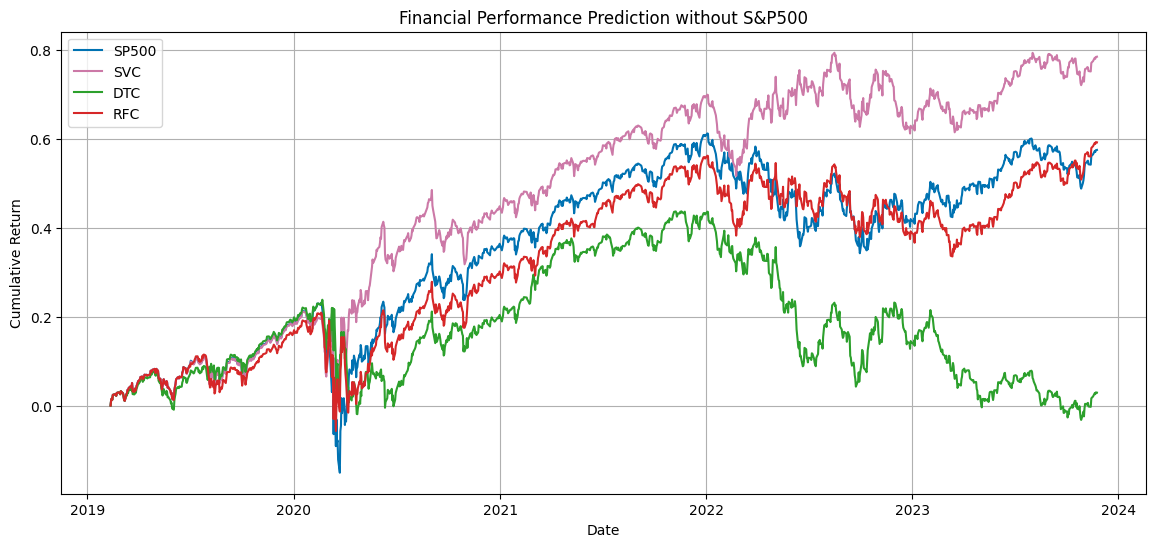
\includegraphics[width=\textwidth]{images/first_visualization.png}
  \end{center}
  \caption[Model return comparison]{Cumulative returns of all three models compared to the long only S\&P500.}
  \label{fig: cumulative returns}
\end{figure}



\begin{figure}[h!]
    \centering
    \animategraphics[loop,autoplay,width=\linewidth]{4}{images/financial_performance_animation-}{0}{19}
    \caption{Cumulative returns for different seeds.}
    \label{fig: moving_returns}
\end{figure}

\section{Simulation}
\label{Simulation}

In order to get a more robust understanding of the way our models perform, we perform a simulation. Our simulation function accepts various parameters to customize the simulations, including the dataset, selected currencies, S\&P 500 inclusion, lag time, training dataset size, and the choice to focus on long-only strategies. The function also allows for the user to vary the number of simulations to run. Next we plot our simulation results, which can be seen below. Here we plot results from running 250 simulations. 
\newline
\indent In order to visualise our results we calculate various quantiles. For the RFC and DTC models, it calculates the 25th, 50th (median), and 75th quantiles for the last simulation's results. We then plot cumulative results for the various machine learning techniques, highlighting the different quantiles and comparing them to the S\&P 500 performance. Crucial to note is that for the SVM, due to its simple architecture and it being a categorisation problem, despite changing the seed, there is only 1 possible path. Therefore each simulation yields the same path. Below we therefore plot the results from this simulation for the DTC and RFC.
\begin{figure}[h!]
\begin{center}
  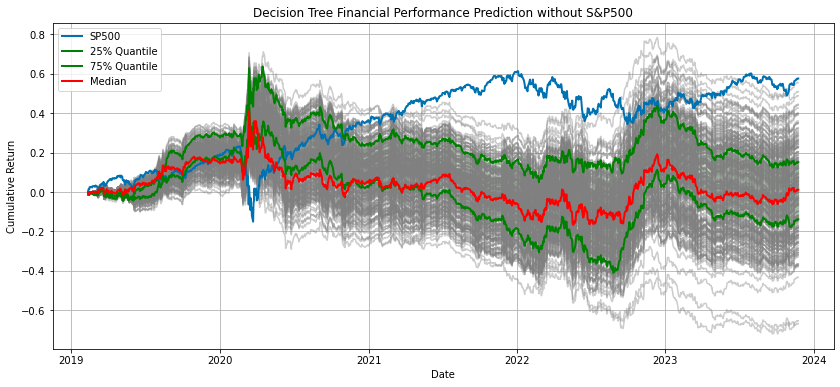
\includegraphics[width=\textwidth]{images/dt_sim.png}
  \end{center}
  \caption[Simulated results for Decision Trees]{Simulated results for Decision Trees}
  \label{fig: DTC simulated returns}
\end{figure}

\begin{figure}[h!]
\begin{center}
  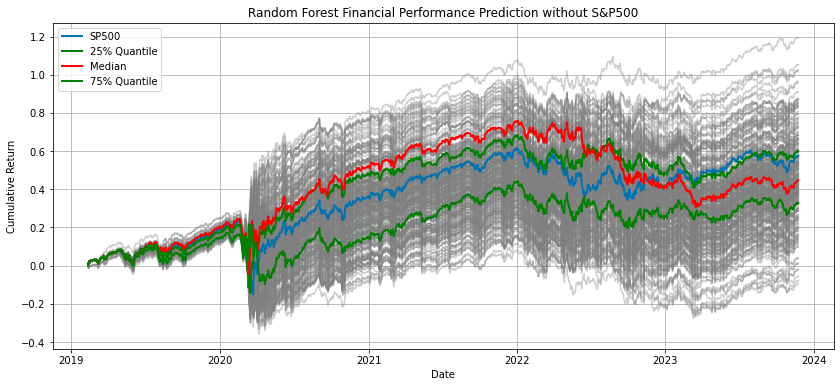
\includegraphics[width=\textwidth]{images/rf_sim.png}
  \end{center}
  \caption[Simulated results for Random Forests]{Simulated results for Random Forests}
  \label{fig: RFC simulated returns}
\end{figure}

What figures \ref{fig: DTC simulated returns} and \ref{fig: RFC simulated returns} show is that the decision trees perform significantly better than the random forest. The median performance is similar to that of the S\&P 500, and the upper quartile performance is actually greater than the S\&P 500 performance. What the simulations show is that there is also a wide range in performance depening on the run. From negative all the way to 100\% cumulative returns. Therefore this shows that there is a lack of stability and in further research, work should be done in order to address this.

\section{Finding the best predictor}
\label{Finding the best predictor}
Another way to analyse the data is to check the behavior in different settings. For this part, we use support vector machines to compare all possible combinations of predicting currencies. That means, we let the model be trained and tested on these currencies as explaining variable. With a total of ten different currencies, this mean that we end up with 1'023 combinations when applying the following formula:

\begin{align}
    C(n) = \sum_{k=1}^{n} \binom{n}{k}
\end{align}

where $n=10$.

\noindent Looking at the results in figure \ref{fig: cumulative returns best predictor}, one cannot detect a real trend again. The best predicting currencies are EUR, JPY, CAD, SEK and SGD together, leading to the highest cumulative return over the testing period with 114\%, but most of the performance is coming from being short S\&P500 during COVID in 2020. 

\begin{figure}[h!]
\begin{center}
  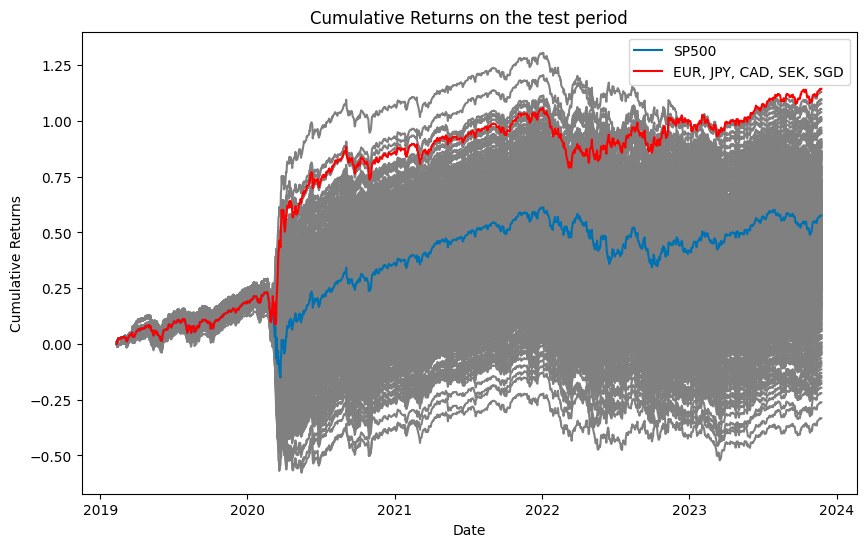
\includegraphics[width=\textwidth]{images/best_predictor.png}
  \end{center}
  \caption[Cumulative returns of all currency combinations]{Cumulative returns of all different combinations used a explanatory variables.}
  \label{fig: cumulative returns best predictor}
\end{figure}

\noindent Let us analyse the top 25 prediction currency combinations. First, we look at the in-sample and out-of-sample errors. The following table \ref{tab:combination_performance} shows the in-sample and out-of-sample accuracies of these combinations. As one can see, the accuracies are not significantly above the mean, which is calculated over the full data. Looking at this table, one can clearly see that some currencies appear more than others. This is visualized in figure \ref{fig: combination_counts}, leading to the EUR being most likely the 'best predictor'.


\begin{table}[h!]
  \centering
  \begin{tabular}{lccc}
    \hline
    Combination & In-Sample & Out-of-Sample \\
    \hline
    EUR, JPY, SEK & 0.545970 & 0.515101 \\
    EUR, GBP, AUD & 0.549748 & 0.523490 \\
    JPY, SEK, SGD & 0.549538 & 0.518456 \\
    EUR, JPY, CAD, SEK & 0.555835 & 0.505034 \\
    EUR, JPY, NZD, SEK & 0.561503 & 0.505034 \\
    EUR, CHF, NZD, NOK & 0.549748 & 0.520973 \\
    JPY, CHF, SEK, NOK & 0.551427 & 0.521812 \\
    JPY, CAD, SEK, SGD & 0.557095 & 0.510067 \\
    GBP, CHF, AUD, NZD & 0.551008 & 0.526846 \\
    EUR, JPY, GBP, CAD, SEK & 0.565911 & 0.499161 \\
    EUR, JPY, AUD, NZD, SEK & 0.562133 & 0.515101 \\
    EUR, JPY, CAD, NZD, SEK & 0.565281 & 0.496644 \\
    EUR, JPY, CAD, SEK, SGD & 0.561713 & 0.510906 \\
    EUR, GBP, CHF, AUD, NZD & 0.556255 & 0.526846 \\
    EUR, CHF, AUD, NZD, SEK & 0.555416 & 0.520973 \\
    EUR, CHF, AUD, NZD, NOK & 0.554156 & 0.529362 \\
    EUR, CHF, CAD, NZD, NOK & 0.558144 & 0.520134 \\
    EUR, AUD, CAD, NZD, SEK & 0.561293 & 0.520973 \\
    EUR, CAD, NZD, SEK, SGD & 0.561923 & 0.515940 \\
    GBP, AUD, CAD, NZD, SGD & 0.558564 & 0.513423 \\
    EUR, JPY, CHF, CAD, SGD, NOK & 0.560873 & 0.515940 \\
    EUR, GBP, CHF, CAD, NZD, SEK & 0.567380 & 0.508389 \\
    EUR, CHF, AUD, NZD, SEK, NOK & 0.557095 & 0.529362 \\
    EUR, CHF, CAD, NZD, SGD, NOK & 0.565281 & 0.520134 \\
    EUR, JPY, GBP, CAD, NZD, SGD, NOK & 0.573468 & 0.500000 \\
    \hline
    \textbf{mean}  & \textbf{0.558522} & \textbf{0.509974}
  \end{tabular}
  \caption{In-Sample and Out-of-Sample Performance for best 25 combinations. }
  \label{tab:combination_performance}
\end{table}

\newpage

\begin{figure}[h]
  \centering
  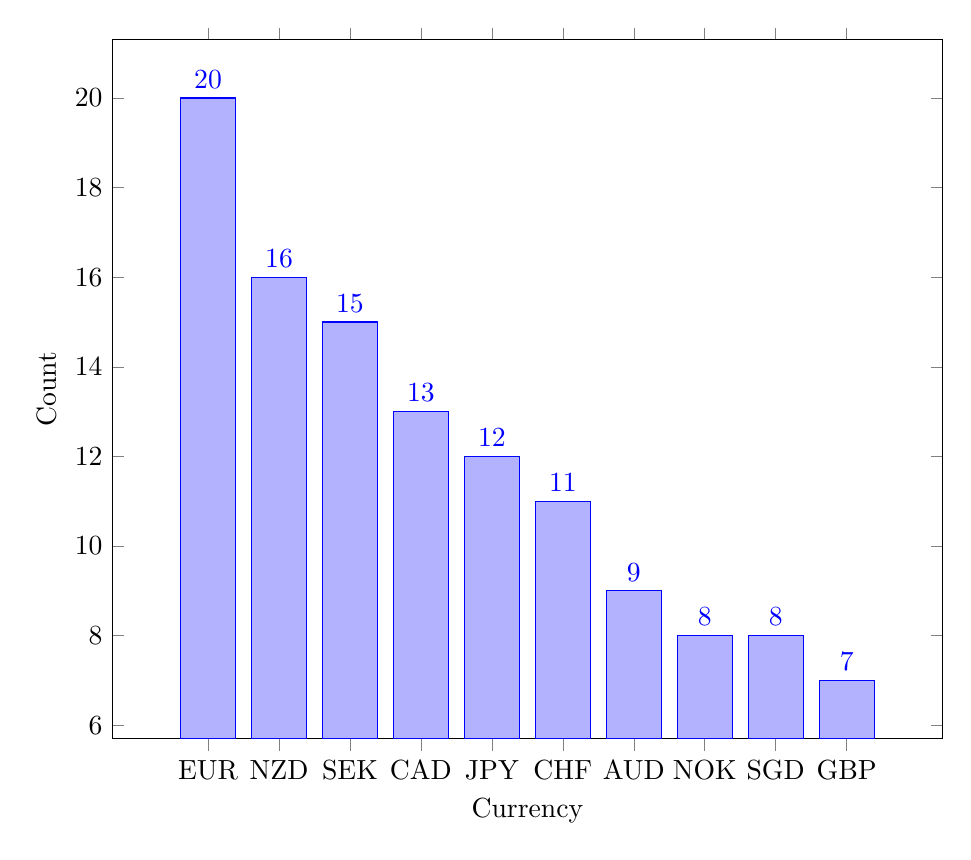
\begin{tikzpicture}
    \begin{axis}[
        ybar,
        bar width=0.7cm,
        xlabel={Currency},
        ylabel={Count},
        symbolic x coords={EUR, NZD, SEK, CAD, JPY, CHF, AUD, NOK, SGD, GBP},
        xtick=data,
        enlarge x limits=0.15,
        nodes near coords,
        nodes near coords align={vertical},
        width=\textwidth,  % Set the width to \textwidth
        ]
      \addplot coordinates {
        (EUR, 20)
        (NZD, 16)
        (SEK, 15)
        (CAD, 13)
        (JPY, 12)
        (CHF, 11)
        (AUD, 9)
        (NOK, 8)
        (SGD, 8)
        (GBP, 7)
      };
    \end{axis}
  \end{tikzpicture}
  \caption{Counts for each currency in the top 25 cumulative returns.}
  \label{fig: combination_counts}
\end{figure}

\noindent Checking some statistics for all cases where EUR is included only lead to a mean excess return of 3\% or 0.5\% per annum. So as soon as transaction costs are included for example, or the model is being set up more complicated in another way, like including margin requirements when being short, all this excess return is eaten up. So again, we cannot find a significant relationship between the currency returns and the S\&P500 returns. Also, we seem to confirm the efficient market hypothesis, meaning all information is being included in all markets.

\noindent Finally, to check this statement once more by creating a histogram of the cumulative returns (the end value) in figure \ref{fig: cumreturns histogram}. Comparing the mean with the long S\&P500, one can observe that the mean is below the benchmark.

\begin{figure}[H]
\begin{center}
  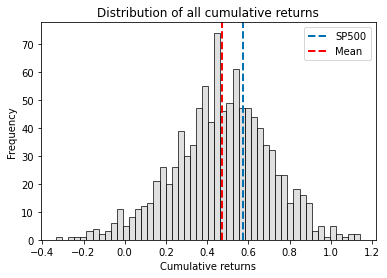
\includegraphics[width=\textwidth]{images/hist_comparison.png}
  \end{center}
  \caption{Cumulative returns distribution of all currency combinations.}
  \label{fig: cumreturns histogram}
\end{figure}


\section{Considerations for future work}
\label{Considerations for future work}
Moving forward, several avenues for further investigation could enhance the depth of our analysis:

\begin{itemize}
    \item Feature Engineering: Explore additional features or alternative representations of currency data that may capture nuances overlooked in the initial analysis. This could involve considering derivatives or transformations of the existing data to unveil hidden patterns.
    \item Model Complexity: Experiment with more sophisticated machine learning models or ensemble methods that may better capture non-linear relationships within the data. Additionally, consider refining hyperparameters or incorporating other relevant financial indicators to enhance predictive accuracy.
    \item Data Granularity: Assess whether utilizing higher-frequency data or incorporating intraday trading signals could uncover more nuanced patterns that might be obscured in daily or monthly aggregates.
    \item Macro-Economic Indicators: Integrate macroeconomic indicators beyond currency data, such as interest rates, inflation, or geopolitical events, to assess their impact on S\&P 500 returns. This holistic approach may reveal interconnected relationships that contribute to predictive power.
    \item Ensemble Strategies: Explore ensemble strategies that combine the strengths of multiple models or incorporate different sources of information. This approach may provide a more robust framework for predicting S\&P 500 returns.
    \item Extended Timeframes: Extend the analysis over a more extended period to assess the models' performance under diverse market conditions and to capture longer-term trends that may not be apparent in shorter timeframes.
\end{itemize}

By delving deeper into these aspects, we can refine our understanding of the interplay between currency data and S\&P 500 returns, potentially identifying subtle patterns or relationships that were not evident in the initial analysis. Remember, the dynamic nature of financial markets necessitates a multifaceted and adaptive approach to uncover meaningful insights.

\section{Conclusion}
\label{Conclusion}
In conclusion, our comprehensive analysis utilizing decision tree, random forest, and support vector machines did not reveal any significant inefficiencies that would suggest a reliable predictive relationship between currency data and S\&P 500 returns. In our exploration of the support vector machine (SVM) model, we identified the Euro (EUR) as the most effective currency in terms of prediction, albeit with a marginal outperformance of approximately 3\% over a 4.7-year out-of-sample (OOS) period. While this may suggest some predictive power, the limited magnitude of the outperformance raises questions about the practical significance of such findings in the context of a dynamic and complex financial landscape. Despite conducting simulations, the cumulative returns appeared to exhibit a random pattern, indicating that the models failed to consistently outperform the market.
